% CS615 Aspects of System Administration
% Author: Jan Schaumann <jschauma@netmeister.org>
% $Id: slides.tex,v 1.6 2006/03/07 13:55:55 jschauma Exp $

\documentclass[xga]{xdvislides}
\usepackage[landscape]{geometry}
\usepackage{graphics}
\usepackage{graphicx}
\usepackage{colordvi}

\begin{document}
\setfontphv

%%% Headers and footers
\lhead{\slidetitle}                               % default:\lhead{\slidetitle}
\chead{CS615 - Aspects of System Administration}% default:\chead{\relax}
\rhead{Slide \thepage}                       % default:\rhead{\sectiontitle}
\lfoot{\Gray{DNS; Backup and Disaster Recovery}}% default:\lfoot{\slideauthor}
\cfoot{\relax}                               % default:\cfoot{\relax}
\rfoot{\Gray{\today}}

\newcommand{\smallish}{\fontsize{15}{20}\selectfont}

\vspace*{\fill}
\begin{center}
	\Hugesize
		CS615 - Aspects of System Administration\\ [1em]
		DNS; Backup and Disaster Recovery \\ [1em]
	\hspace*{5mm}\blueline\\ [1em]
	\Normalsize
		Department of Computer Science\\
		Stevens Institute of Technology\\
		Jan Schaumann\\
		\verb+jschauma@stevens-tech.edu+
		\verb+http://www.cs.stevens-tech.edu/~jschauma/615A/+
\end{center}
\vspace*{\fill}

\subsection{In the beginning...}
\vspace*{\fill}
\begin{center}
	\includegraphics[scale=0.8]{pics/2computers.eps} \\
\end{center}
\vspace*{\fill}

\subsection{In the beginning...}
\vspace*{\fill}
\begin{center}
	\includegraphics[scale=0.8]{pics/2computers-nic.eps} \\
\end{center}
\vspace*{\fill}

\subsection{In the beginning...}
\vspace*{\fill}
\begin{center}
	\includegraphics[scale=0.8]{pics/3computers.eps} \\
\end{center}
\vspace*{\fill}

\subsection{In the beginning...}
\vspace*{\fill}
\begin{center}
	\includegraphics[scale=0.8]{pics/3computers-1.eps} \\
\end{center}
\vspace*{\fill}

\subsection{In the beginning...}
\vspace*{\fill}
\begin{center}
	\includegraphics[scale=0.8]{pics/3computers-2.eps} \\
\end{center}
\vspace*{\fill}

\subsection{In the beginning...}
\vspace*{\fill}
\begin{center}
	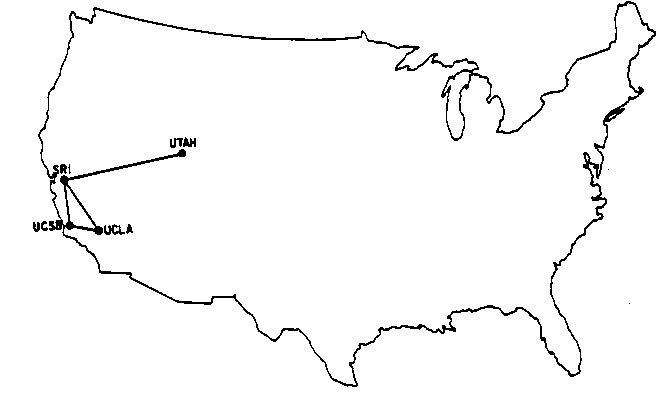
\includegraphics[scale=0.8]{pics/arpanet1.eps} \\
\end{center}
\vspace*{\fill}


\subsection{In the beginning...}
\begin{verbatim}
# Host Database
# This file should contain the addresses and aliases
# for local hosts that share this file.
#
127.0.0.1               localhost localhost.
#
# RFC 1918 specifies that these networks are "internal".
# 10.0.0.0      10.255.255.255
# 172.16.0.0    172.31.255.255
# 192.168.0.0   192.168.255.255
10.0.0.1	UCLA-TEST
10.0.0.2	SRI-SPRM
10.0.0.4	UTAH-CS
\end{verbatim}


\subsection{But then...}
\vspace*{\fill}
\begin{center}
	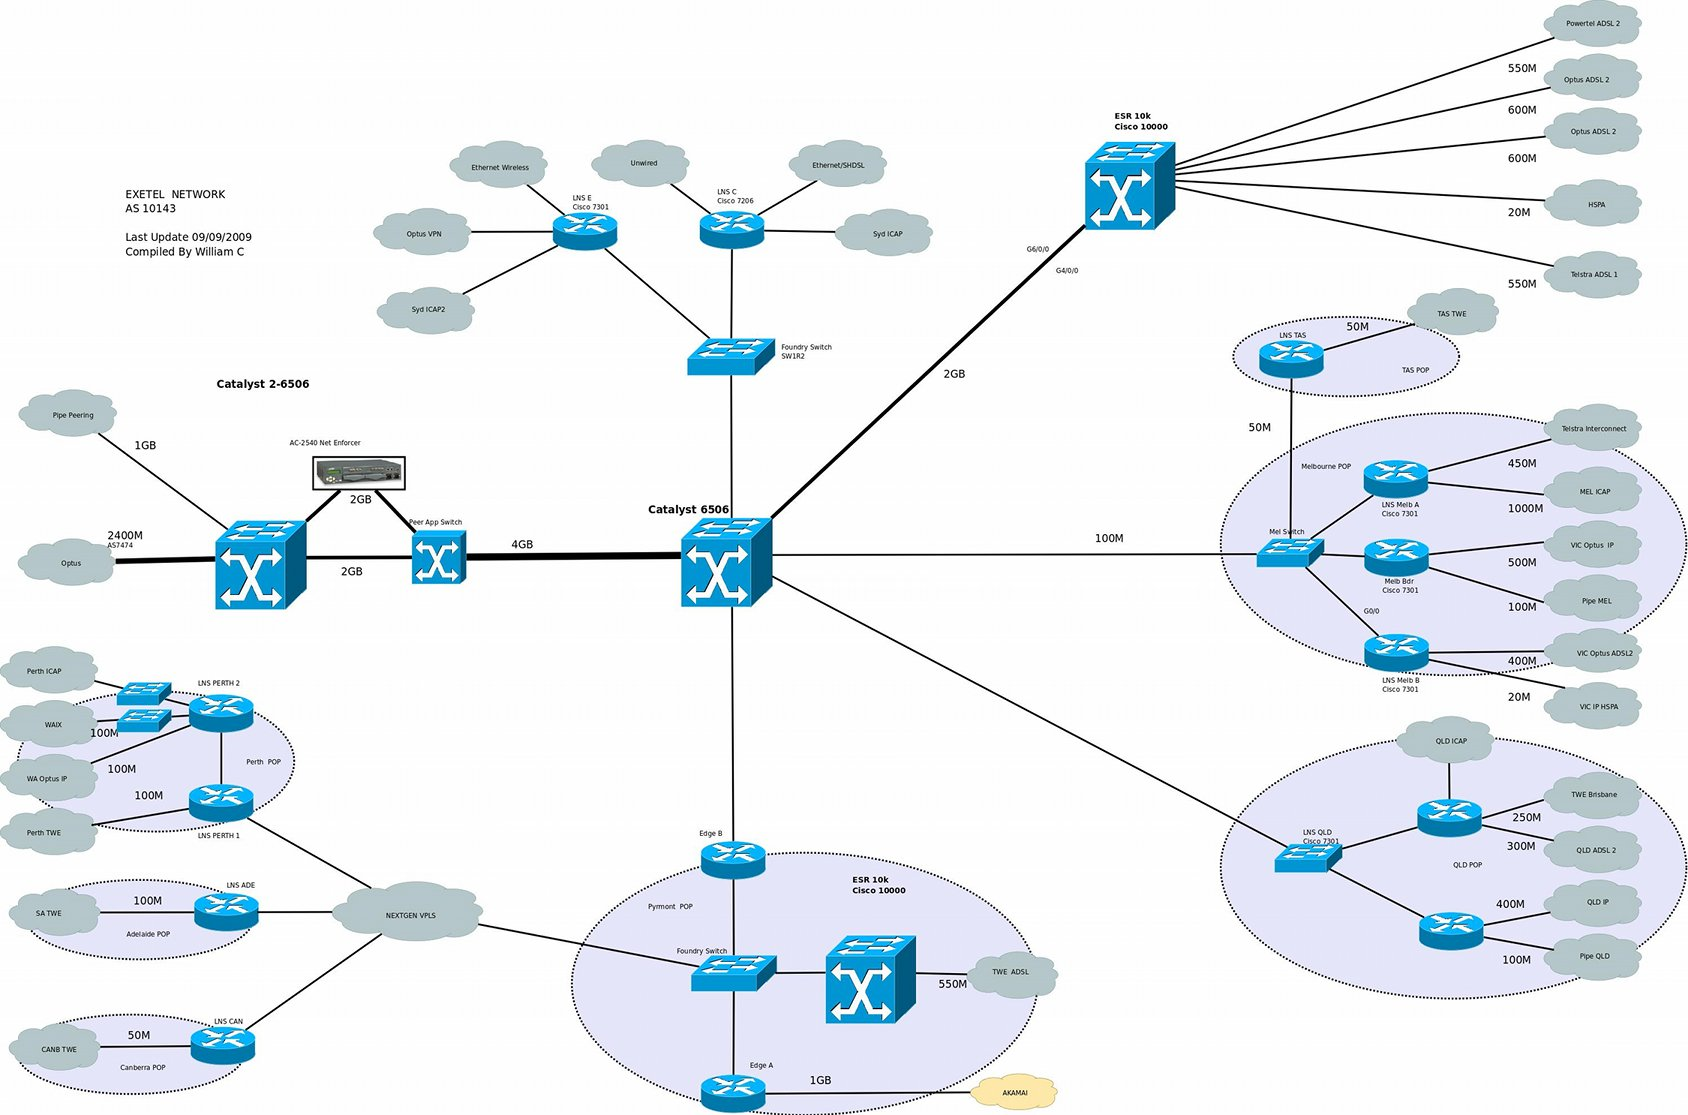
\includegraphics[scale=0.3]{pics/routed.eps} \\
\end{center}
\vspace*{\fill}

\subsection{The Domain Name System}
\vspace{.5in}
\begin{center}
	\Huge
	Computers like numbers. \\
\vspace{.5in}
\begin{verbatim}
         10011011111101100101100110011111
\end{verbatim}
\end{center}
\Normalsize

\subsection{The Domain Name System}
\vspace{.5in}
\begin{center}
	\Huge
	Computers like numbers. \\
\vspace{.5in}
\begin{verbatim}
      10011011  11110110  01011001  10011111

        155   .   246   .    89   .   159
\end{verbatim}
\end{center}
\Normalsize

\subsection{The Domain Name System}
\vspace{.5in}
\begin{center}
	\Huge
	People like names. \\
\vspace{.5in}
\verb+ash.cs.stevens-tech.edu+
\end{center}
\Normalsize


\subsection{The Domain Name System}
\vspace*{\fill}
\begin{center}
	
\includegraphics[scale=0.6]{pics/phonebook.eps}
\end{center}
\vspace*{\fill}

\subsection{The New Phonebook is here!}
\vspace*{\fill}
\begin{center}
	\verb+http://is.gd/XXp2sC+ \\
	\addvspace{.5in}
	\verb+wget -q -O - http://is.gd/XXp2sC | grep -c "^HOST"+
\end{center}
\vspace*{\fill}

\subsection{DNS: A distributed database}
\vspace*{\fill}
\begin{center}
	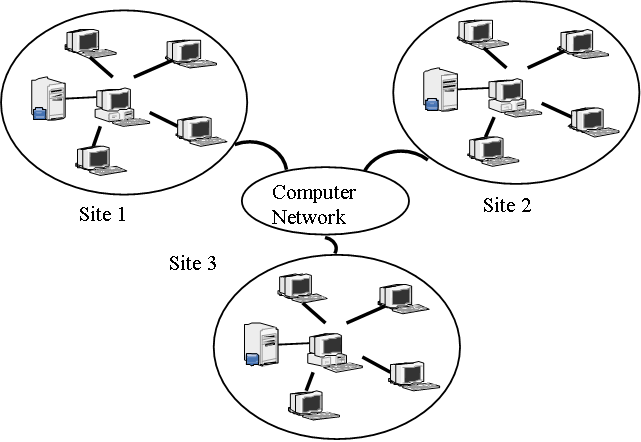
\includegraphics[scale=0.75]{pics/distributed-database.eps}
\end{center}
\vspace*{\fill}

\subsection{The Domain Name Space}
\vspace{.5in}
\begin{center}
	\Huge
	The domain name space consists of a tree of {\em domain} names.
\end{center}
\Normalsize

\subsection{DNS: A hierarchical system}
\vspace*{\fill}
\begin{center}
	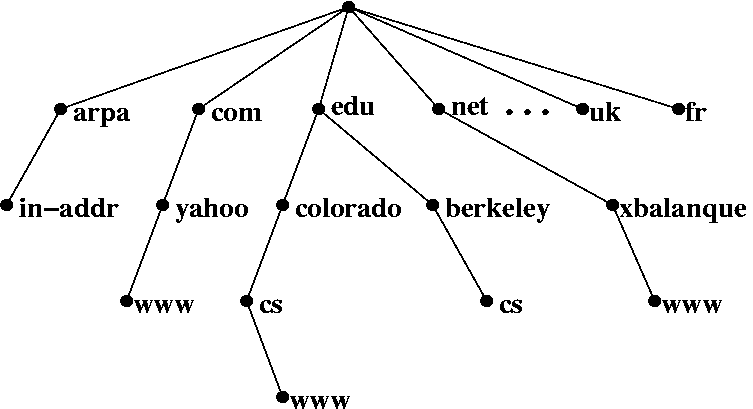
\includegraphics[scale=0.75]{pics/hierarchical-dns.eps}
\end{center}
\vspace*{\fill}

\subsection{The Domain Name Space}
\vspace{.5in}
\begin{center}
	\Huge
	The domain name space consists of a tree of {\em domain} names. \\
	\vspace{.5in}
	A subtree divides into {\em zones}.
\end{center}
\Normalsize

\subsection{The Domain Name Space}
\vspace{.5in}
\begin{center}
	\Huge
	The domain name space consists of a tree of {\em domain} names. \\
	\vspace{.5in}
	A subtree divides into {\em zones}. \\
	\vspace{.5in}
	Each node may contain {\em resource records}.
\end{center}
\Normalsize

\subsection{The Domain Name Space}
\vspace*{\fill}
\begin{center}
	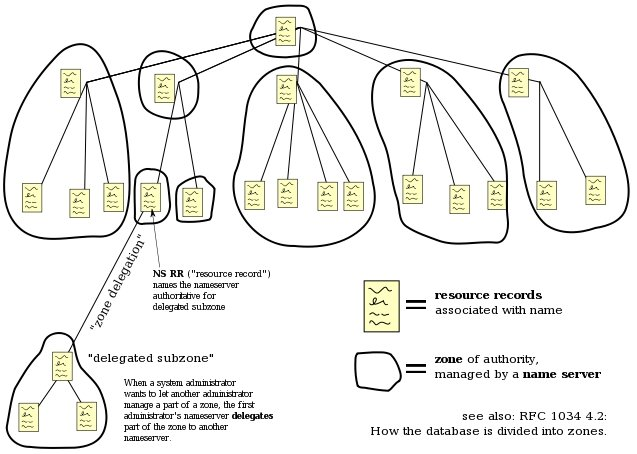
\includegraphics[scale=0.74]{pics/dns-space.eps}
\end{center}
\vspace*{\fill}

\subsection{Domain Names}
\vspace{.5in}
\begin{center}
	\Huge
	\verb+ash.cs.stevens-tech.edu+ \\
	\vspace{.5in}
	Domain Names are read from right to left and components separated by a ``\verb+.+''.
\end{center}
\Normalsize

\subsection{Domain Names}
\vspace{.5in}
\begin{center}
	\Huge
	\verb+ash.cs.stevens-tech.edu.+ \\
	\vspace{.5in}
	The {\em root} is known as ``\verb+.+'', but is usually left out.
\end{center}
\Normalsize

\subsection{Domain Names}
\vspace{.5in}
\begin{center}
	\Huge
	\verb+ash.cs.stevens-tech.+{\bf edu}\verb+.+ \\
	\vspace{.5in}
	There is a small number of {\em top level domains}.
\end{center}
\Normalsize

\subsection{Domain Names}
\vspace{.5in}
\begin{center}
	\Huge
	\verb+ash.cs.stevens-tech.+{\bf edu}\verb+.+ \\
	\vspace{.5in}
	There is a number of {\em top level domains}. \\
	\vspace{.5in}
	\Normalsize
	\begin{verbatim}
wget -O - ftp://rs.internic.net/domain/root.zone | \
        grep "IN<tab>*NS<tab>" | awk '{print $1}' | sort -u | wc -l
\end{verbatim}
	\vspace{.25in}
	\verb+http://data.iana.org/TLD/tlds-alpha-by-domain.txt+ \\
	\verb+https://en.wikipedia.org/wiki/List_of_Internet_top-level_domains+
\end{center}
\Normalsize


\subsection{Domain Names}
\vspace{.5in}
\begin{center}
	\Huge
	\verb+ash.cs.+{\bf stevens-tech}\verb+.edu.+ \\
	\vspace{.5in}
	Each {\em domain} can be divided into any number of {\em sub domains}.
\end{center}
\Normalsize

\subsection{Domain Names}
\vspace{.5in}
\begin{center}
	\Huge
	\verb+ash.+{\bf cs}\verb+.stevens-tech.edu.+ \\
	\vspace{.5in}
	Each {\em domain} can be divided into any number of {\em sub domains}.
\end{center}
\Normalsize

\subsection{Domain Names}
\vspace{.5in}
\begin{center}
	\Huge
	{\bf ash}\verb+.cs.stevens-tech.edu.+ \\
	\vspace{.5in}
	The left-most component of a domain name may be a {\em hostname}.
\end{center}
\Normalsize

\subsection{Fully Qualified Domain Names}
\vspace{.5in}
\begin{center}
	\Huge
	\verb+ash.cs.stevens-tech.edu.+ \\
	\vspace{.5in}
	A {\em hostname} with a domain name is known as a {\em FQDN}.
\end{center}
\Normalsize


\subsection{DNS servers come in two flavors}
\vspace*{\fill}
\begin{center}
	\begin{tabular}{ c c c }
	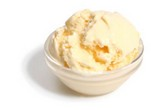
\includegraphics[scale=1.5]{pics/vanilla.eps} & \hspace{.5in} & 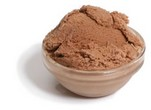
\includegraphics[scale=1.5]{pics/chocolate.eps} \\
	\hspace{.3in} \Huge Authoritative & & \hspace{.3in} \Huge Recursive \\
	\hspace{.3in} \Huge Nameservers & & \hspace{.3in} \Huge Nameservers \\
	\end{tabular}
\end{center}
\vspace*{\fill}

\subsection{Hostname resolution}
Resolution on a recursive nameserver (aka {\em resolver}) involves a number of queries:
\vspace{.5in}
\begin{verbatim}
$ nslookup ash.cs.stevens-tech.edu
Server:         127.0.0.1
Address:        127.0.0.1#53

Non-authoritative answer:
Name:   ash.cs.stevens-tech.edu
Address: 155.246.89.159

$
\end{verbatim}

\subsection{Hostname resolution}
Resolution on a {\em resolver} involves a number of queries:
\begin{verbatim}
18:39:27.186778 IP panix.netmeister.org.62105 > i.root-servers.net.domain:
        11585 [1au] A? ash.cs.stevens-tech.edu. (52)
18:39:27.446190 IP i.root-servers.net.domain > panix.netmeister.org.62105:
        11585- 0/8/8 (494)
18:39:27.446994 IP panix.netmeister.org.53168 > a.gtld-servers.net.domain:
        46575 [1au] A? ash.cs.stevens-tech.edu. (52)
18:39:27.481565 IP a.gtld-servers.net.domain > panix.netmeister.org.53168:
        46575- 0/6/3 (609)
18:39:27.481998 IP panix.netmeister.org.41071 > nrac.stevens-tech.edu.domain:
        24322 [1au] A? ash.cs.stevens-tech.edu. (52)
18:39:27.486035 IP nrac.stevens-tech.edu.domain > panix.netmeister.org.41071:
        24322*- 1/2/3 A[|domain]
\end{verbatim}
\Normalsize

\subsection{Hostname resolution}
Resolution on a {\em resolver} involves a number of queries:
\begin{verbatim}
$ host -t ns .
. name server I.ROOT-SERVERS.NET.
. name server D.ROOT-SERVERS.NET.
. name server C.ROOT-SERVERS.NET.
. name server M.ROOT-SERVERS.NET.
. name server F.ROOT-SERVERS.NET.
. name server A.ROOT-SERVERS.NET.
. name server E.ROOT-SERVERS.NET.
. name server L.ROOT-SERVERS.NET.
. name server H.ROOT-SERVERS.NET.
. name server J.ROOT-SERVERS.NET.
. name server B.ROOT-SERVERS.NET.
. name server G.ROOT-SERVERS.NET.
. name server K.ROOT-SERVERS.NET.
$
\end{verbatim}

\subsection{Hostname resolution}
Resolution on a {\em resolver} involves a number of queries:
\begin{verbatim}
$ dig -t ns edu.
[...]
;; ANSWER SECTION:
edu.                    172800  IN      NS      l.edu-servers.net.
edu.                    172800  IN      NS      f.edu-servers.net.
edu.                    172800  IN      NS      c.edu-servers.net.
edu.                    172800  IN      NS      g.edu-servers.net.
edu.                    172800  IN      NS      a.edu-servers.net.
edu.                    172800  IN      NS      d.edu-servers.net.

;; ADDITIONAL SECTION:
c.edu-servers.net.      36626   IN      A       192.26.92.30
d.edu-servers.net.      13274   IN      A       192.31.80.30
l.edu-servers.net.      36626   IN      A       192.41.162.30
[...]
$
\end{verbatim}
\Normalsize

\subsection{Hostname resolution}
Resolution on a {\em resolver} involves a number of queries:
\begin{verbatim}
$ dig @c.edu-servers.net -t ns stevens.edu.
[...]
;; AUTHORITY SECTION:
stevens.edu.            172800  IN      NS      nrac.stevens-tech.edu.
stevens.edu.            172800  IN      NS      sitult.stevens-tech.edu.

;; ADDITIONAL SECTION:
nrac.stevens-tech.edu.  172800  IN      A       155.246.1.21
sitult.stevens-tech.edu. 172800 IN      A       155.246.1.20
[...]
$
\end{verbatim}

\subsection{Hostname resolution}
\vspace*{\fill}
\begin{center}
	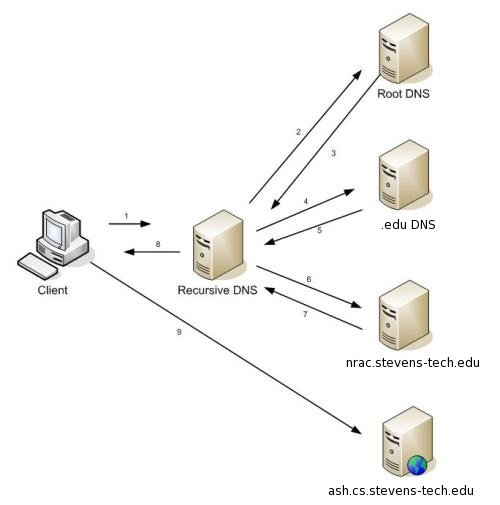
\includegraphics[scale=0.9]{pics/resolution.eps}
\end{center}
\vspace*{\fill}


\subsection{Hostname resolution}
Resolution on a {\em resolver} involves a number of queries:
\begin{verbatim}
$ nslookup ash.cs.stevens-tech.edu
Server:         127.0.0.1
Address:        127.0.0.1#53

Non-authoritative answer:
Name:   ash.cs.stevens-tech.edu
Address: 155.246.89.159

$
\end{verbatim}

\subsection{Hostname resolution}
\vspace*{\fill}
\begin{center}
	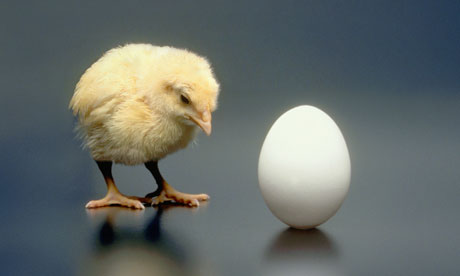
\includegraphics[scale=0.4]{pics/chicken-egg.eps} \\
	\vspace*{\fill}
\end{center}

\subsection{Hostname resolution}
\vspace*{\fill}
\begin{center}
	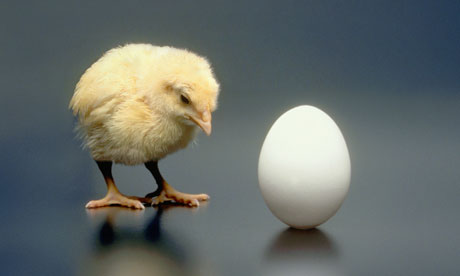
\includegraphics[scale=0.4]{pics/chicken-egg.eps} \\
	\addvspace{.2in}
	\verb+$ ftp -o - ftp.internic.net:/domain/db.cache | more+ \\
	\verb+http://www.internic.net/zones/named.root+
	\vspace*{\fill}
\end{center}

\subsection{Operation Global Blackout}
\vspace*{\fill}
\begin{center}
	
\includegraphics[scale=0.8]{pics/anonymous.eps} \\
	\addvspace{.2in}
	\verb+http://pastebin.com/XZ3EGsbc+ \\
	\addvspace{.1in}
\end{center}
\vspace*{\fill}

\subsection{DNS: A distributed system}
\vspace{.5in}
\begin{center}
	\Huge
	There are 13 \verb+root+ servers. \\
\end{center}
\Normalsize

\subsection{DNS: A distributed system}
\vspace{.5in}
\begin{center}
	\Huge
	There are 13 \verb+root+ servers. \\
	\vspace{.5in}
	Except... there are more.
\end{center}
\Normalsize

\subsection{DNS: A distributed system}
\vspace{.5in}
\begin{center}
	\Huge
	There are 13 \verb+root+ {\em authorities}. \\
\end{center}
\Normalsize

\subsection{DNS: A distributed system}
\vspace{.5in}
\begin{center}
	\Huge
	There are 13 \verb+root server+ {\em addresses}. \\
\end{center}
\Normalsize

\subsection{DNS: A distributed system}
\vspace{.5in}
\begin{center}
	\Huge
	There are hundreds of \verb+root+ servers. \\
\end{center}
\Normalsize

\subsection{DNS: A distributed system}
\vspace*{\fill}
\begin{center}
	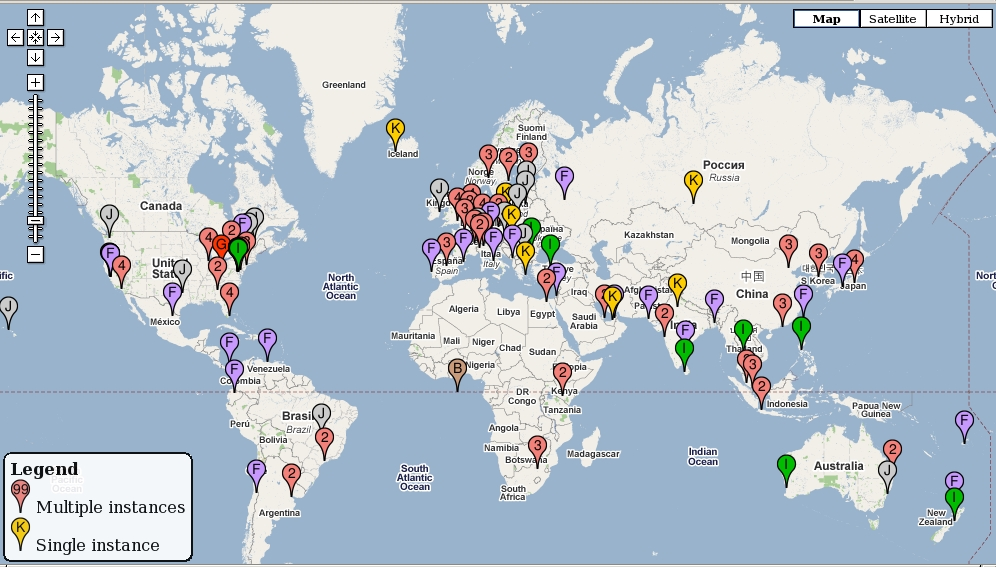
\includegraphics[scale=0.5]{pics/root-servers.eps}
\end{center}
\vspace*{\fill}

\subsection{Operation Global Blackout}
\vspace*{\fill}
\begin{center}
	
\includegraphics[scale=0.8]{pics/anonymous-tweet.eps} \\
\end{center}
\vspace*{\fill}

\subsection{DNS: A distributed database}
\vspace*{\fill}
\begin{center}
	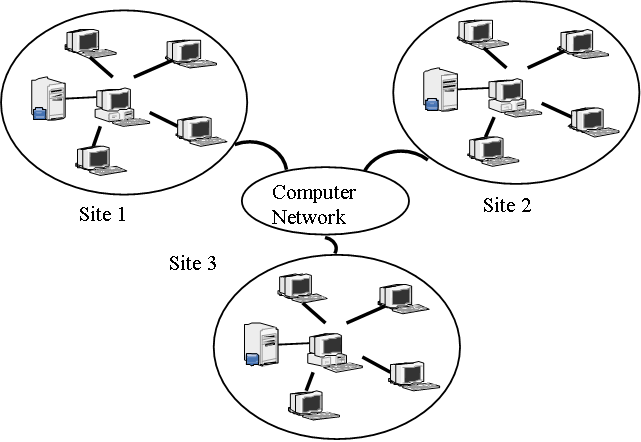
\includegraphics[scale=0.75]{pics/distributed-database.eps}
\end{center}
\vspace*{\fill}


\subsection{DNS Resource Records}
\begin{itemize}
	\item {\em NS} -- an authoritative name server
	\item {\em CNAME} -- the canonical name for an alias
	\item {\em SOA} -- marks the start of a zone of authority
	\item {\em PTR} -- a domain name pointer
	\item {\em HINFO} -- host information
	\item {\em MX} -- mail exchange
	\item {\em TXT} text strings
	\item ...
\end{itemize}

\subsection{DNS Resource Records}
Exercise: trace DNS queries for a reverse lookup (PTR):
\\

\begin{verbatim}
$ host ash.cs.stevens-tech.edu
ash.cs.stevens-tech.edu has address 155.246.89.159
ash.cs.stevens-tech.edu mail is handled by 0 guinness.cs.stevens-tech.edu.
$ host 155.246.89.159
159.89.246.155.in-addr.arpa domain name pointer ash.cs.stevens-tech.edu.
$ 
\end{verbatim}

\subsection{Creative uses of DNS Resource Records}
\begin{itemize}
	\item identifying sources of SPAM
	\item find out if the internet is on fire: \\
		\verb|dig +short txt istheinternetonfire.com|
	\item find ASN numbers by IP addresses: \\
		\verb|dig +short 159.89.246.155.origin.asn.cymru.com TXT|
	\item check a resolver's source port randomization (to help
		mitigate DNS Cache Poisoning attacks): \\
		\verb|dig +short porttest.dns-oarc.net TXT|
	\item using DNS to publish SSH key fingerprints (RFC4255,
ssh\_config(5) \verb+VerifyHostKeyDNS+; for best results combine with DNSSEC): \\
		\verb|dig +short ftp.netbsd.org SSHFP|
		\begin{verbatim}
ssh -o "VerifyHostKeyDNS yes" ftp.netbsd.org
[...]
Matching host key fingerprint found in DNS.
Are you sure you want to continue connecting (yes/no)?
\end{verbatim}
\end{itemize}

\newpage
\vspace*{\fill}
\begin{center}
    \Hugesize
        Hooray! \\ [1em]
    \hspace*{5mm}
    \blueline\\
    \hspace*{5mm}\\
        5 Minute Break
\end{center}
\vspace*{\fill}

\subsection{Backups}
\begin{itemize}
	\item backup vs. restore
\end{itemize}

\subsection{Backups}
\begin{itemize}
	\item backup vs. restore
	\item backup devices and media
\end{itemize}
\vspace*{\fill}
\begin{center}
	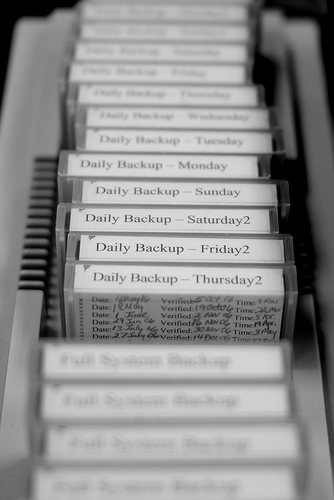
\includegraphics[scale=2.0]{pics/daily-tapes.eps}
\end{center}
\vspace*{\fill}

\subsection{Backups}
\begin{itemize}
	\item backup vs. restore
	\item backup devices and media
\end{itemize}
\vspace*{\fill}
\begin{center}
	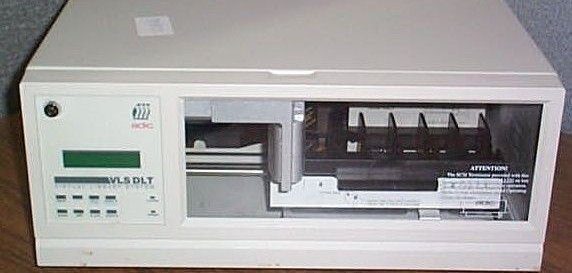
\includegraphics[scale=0.8]{pics/dlt-library.eps}
\end{center}
\vspace*{\fill}

\subsection{Backups}
\begin{itemize}
	\item backup vs. restore
	\item backup devices and media
\end{itemize}
\vspace*{\fill}
\begin{center}
	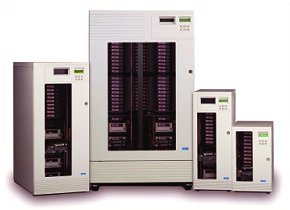
\includegraphics[scale=1.0]{pics/libraries.eps}
\end{center}
\vspace*{\fill}

\subsection{Backups}
\begin{itemize}
	\item backup vs. restore
	\item backup devices and media
	\item filesystem considerations
\end{itemize}

\subsection{Backups}
\begin{itemize}
	\item backup vs. restore
	\item backup devices and media
	\item filesystem considerations
	\item backup strategies
\end{itemize}

\subsection{Backups}
\begin{itemize}
	\item backup vs. restore
	\item backup devices and media
	\item filesystem considerations
	\item backup strategies
	\item planning for disasters
\end{itemize}

\subsection{Backups and Restore Basics}
When do we need backups?

\subsection{Backups and Restore Basics}
When do we need backups?
\begin{itemize}
	\item disaster recovery: off-site storage of sensitive data
	\item long-term storage requirements
	\item recover from data loss
\end{itemize}

\subsection{Backups and Restore Basics}
When do we need backups?
\begin{itemize}
	\item disaster recovery: off-site storage of sensitive data
	\item long-term storage requirements
	\item recover from data loss due to
\end{itemize}
\vspace*{\fill}
\begin{center}
	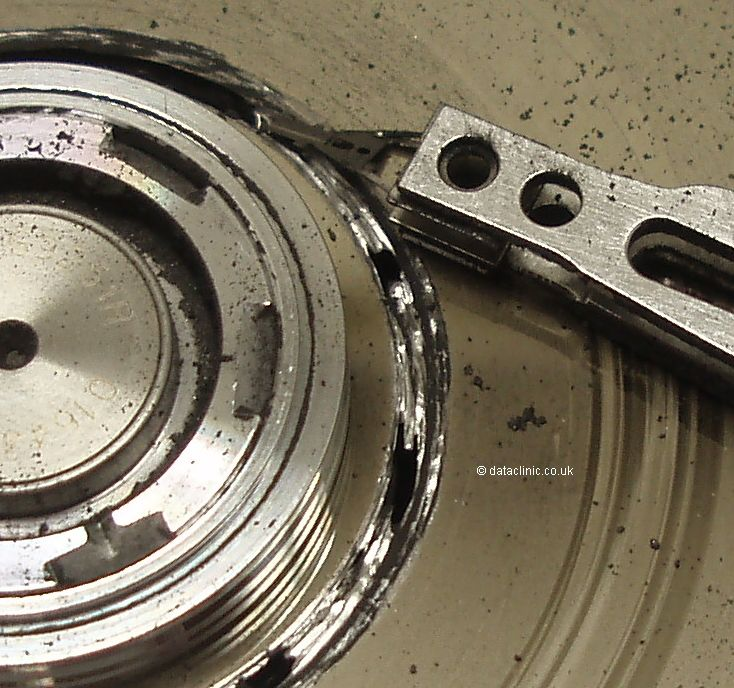
\includegraphics[scale=1.0]{pics/headcrash-closeup.eps}
\end{center}
\vspace*{\fill}

\subsection{Backups and Restore Basics}
When do we need backups?
\begin{itemize}
	\item disaster recovery: off-site storage of sensitive data
	\item long-term storage requirements
	\item recover from data loss due to
\end{itemize}
\vspace*{\fill}
\begin{center}
	
\includegraphics[scale=1.2]{pics/dumb-user.eps}
\end{center}
\vspace*{\fill}

\subsection{Backups and Restore Basics}
When do we need backups?
\begin{itemize}
	\item disaster recovery: off-site storage of sensitive data
	\item long-term storage requirements
	\item recover from data loss due to
\end{itemize}
\vspace*{\fill}
\begin{center}
	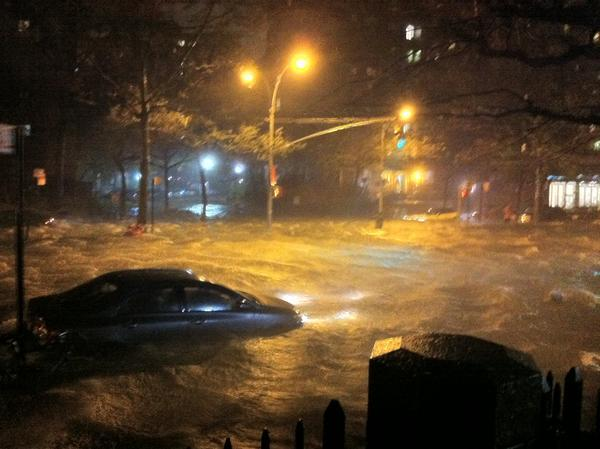
\includegraphics[scale=0.4]{pics/20th-and-C.eps}
\end{center}
\vspace*{\fill}

\subsection{Backups and Restore Basics}
When do we need backups?
\begin{itemize}
	\item disaster recovery: off-site storage of sensitive data
	\item long-term storage requirements
	\item recover from data loss due to
\end{itemize}
\vspace*{\fill}
\begin{center}
	
\includegraphics[scale=0.6]{pics/hacker.eps}
\end{center}
\vspace*{\fill}

\subsection{Backups and Restore Basics}
When do we need backups?
\begin{itemize}
	\item disaster recovery: off-site storage of sensitive data
	\item long-term storage requirements
	\item recover from data loss due to
\end{itemize}
\vspace*{\fill}
\begin{center}
	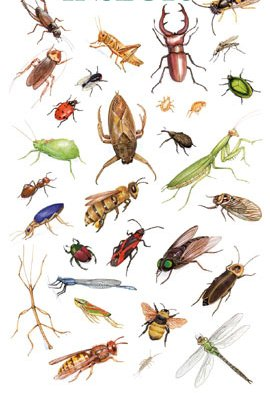
\includegraphics[scale=0.6]{pics/bugs.eps}
\end{center}
\vspace*{\fill}

\subsection{Backups and Restore Basics}
When do we need backups?
\begin{itemize}
	\item disaster recovery: off-site storage of sensitive data
	\item long-term storage requirements
	\item recover from data loss due to
		\begin{itemize}
			\item equipment failure
			\item bozotic users
			\item natural disaster
			\item security breach
			\item software bugs
		\end{itemize}
\end{itemize}

\subsection{Backups and Restore Basics}
When do we need backups?
\begin{itemize}
	\item disaster recovery: off-site storage of sensitive data
	\item long-term storage requirements
	\item recover from data loss due to
		\begin{itemize}
			\item equipment failure
			\item bozotic users
			\item natural disaster
			\item security breach
			\item software bugs
		\end{itemize}
\end{itemize}
\addvspace{.5in}
Think of your backups as {\em insurance}:  you invest and pay for it, hoping
you will never need it.


\subsection{Key Reasons for Restores}
Three key reasons for restores: {\em Accidental File Deletion}, {\em Disk
Failure} and {\em Archival}.
\\

1. Accidental File Deletion
\begin{itemize}
	\item ability to restore a file within a certain time frame
	\item restore time, including
		\begin{itemize}
			\item actual time spent restoring
			\item waiting until resources permit the restore
			\item staff availability
		\end{itemize}
	\item self-service restore
\end{itemize}

\subsection{Key Reasons for Restores}
2. Disk Failure
\begin{itemize}
	\item loss of entire file system
	\item leads to downtime
	\item RAID may help
	\item takes long time to restore
\end{itemize}
\addvspace{.5in}
3. Archival
\begin{itemize}
	\item {\em full} set of level 0 backups
	\item separate set from regular backups
	\item usually stored off-site
	\item store for long time
\end{itemize}

\subsection{Filesystem backup}
{\tt dump(8)} / {\tt restore(8)}
\begin{itemize}
	\item in use since \~{}1975
	\item full filesystem level backups
	\item direct interaction with tape devices
	\item integration with {\tt /etc/fstab}
	\item efficient incremental backups
\end{itemize}

\subsection{Filesystem backup}
\begin{itemize}
	\item start an Ubuntu EC2 instance (e.g. \verb+ami-6de0dd04+)
	\item create a full filesystem backup using \verb+dump(8)+
	\item add the 'apache2' package
	\item create an incremental backup
	\item delete the 'apache2' package
	\item restore all files from the incremental backup using the \verb+restore(8)+ command
	\item verify that the 'apache2' package is fully installed
\end{itemize}

\subsection{Filesystem backup}
\begin{verbatim}
ssh ec2-instance "sudo dump -u -0 -f - /" | bzip2 -c -9 >tmp/ubuntu.0.bz2
  DUMP: Date of this level 0 dump: Thu Mar 26 19:25:06 2015
  DUMP: Dumping /dev/xvda1 (/) to standard output
  DUMP: Label: cloudimg-rootfs
  DUMP: Writing 10 Kilobyte records
  DUMP: mapping (Pass I) [regular files]
  DUMP: mapping (Pass II) [directories]
  DUMP: estimated 823759 blocks.
  DUMP: Volume 1 started with block 1 at: Thu Mar 26 19:25:07 2015
  DUMP: dumping (Pass III) [directories]
  DUMP: dumping (Pass IV) [regular files]
  DUMP: Volume 1 completed at: Thu Mar 26 19:28:21 2015
  DUMP: Volume 1 820690 blocks (801.46MB)
  DUMP: Volume 1 took 0:03:14
  DUMP: Volume 1 transfer rate: 4230 kB/s
  DUMP: 820690 blocks (801.46MB)
  DUMP: finished in 194 seconds, throughput 4230 kBytes/sec
  DUMP: Date of this level 0 dump: Thu Mar 26 19:25:06 2015
  DUMP: Date this dump completed:  Thu Mar 26 19:28:21 2015
  DUMP: Average transfer rate: 4230 kB/s
  DUMP: DUMP IS DONE
\end{verbatim}


\subsection{Filesystem backup}
\begin{verbatim}
$ cat /var/lib/dumpdates 
/dev/xvda1 0 Thu Mar 26 19:25:06 2015 +0000
$ sudo apt-get install apache2
[...]
$ ssh ec2-instance "sudo dump -u -1 -f - /" | bzip2 -c -9 >tmp/ubuntu.1.bz2
  DUMP: Date of this level 2 dump: Thu Mar 26 19:56:45 2015
  DUMP: Date of last level 1 dump: Thu Mar 26 19:48:58 2015
  DUMP: Dumping /dev/xvda1 (/) to standard output
  DUMP: Label: cloudimg-rootfs
  DUMP: Writing 10 Kilobyte records
  DUMP: mapping (Pass I) [regular files]
  DUMP: mapping (Pass II) [directories]
  DUMP: estimated 39644 blocks.
  DUMP: Volume 1 started with block 1 at: Thu Mar 26 19:56:50 2015
  DUMP: dumping (Pass III) [directories]
  DUMP: dumping (Pass IV) [regular files]
  DUMP: Volume 1 completed at: Thu Mar 26 19:56:56 2015
  DUMP: Volume 1 39820 blocks (38.89MB)
  DUMP: Volume 1 took 0:00:06
  DUMP: Volume 1 transfer rate: 6636 kB/s
  DUMP: 39820 blocks (38.89MB)
  DUMP: finished in 5 seconds, throughput 7964 kBytes/sec
  DUMP: Date of this level 2 dump: Thu Mar 26 19:56:45 2015
  DUMP: Date this dump completed:  Thu Mar 26 19:56:56 2015
  DUMP: Average transfer rate: 6636 kB/s
  DUMP: DUMP IS DONE
\end{verbatim}

\subsection{Filesystem backup}
\vspace*{\fill}
\begin{center}
	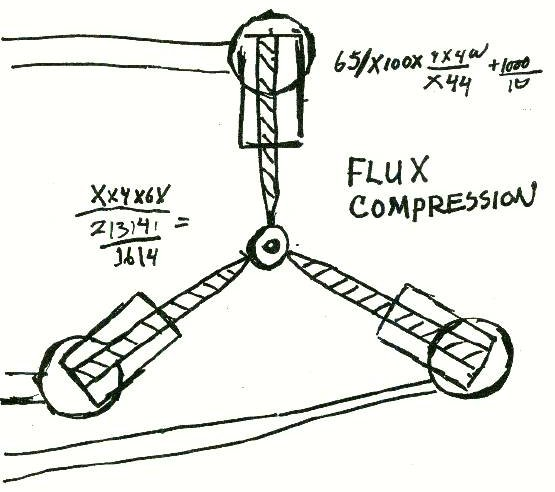
\includegraphics[scale=0.7]{pics/flux-capacitor.eps}
\end{center}
\vspace*{\fill}

\subsection{Filesystem backup}
\vspace*{\fill}
\begin{center}
	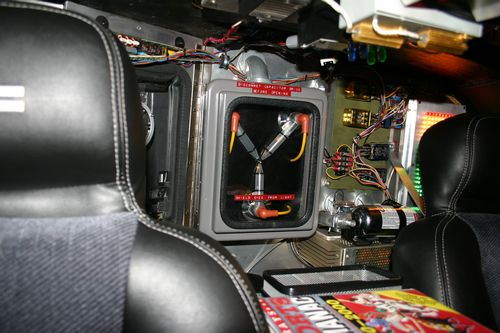
\includegraphics[scale=2.5]{pics/flux-capacitor2.eps}
\end{center}
\vspace*{\fill}

\subsection{Filesystem backup}
\vspace*{\fill}
\begin{center}
	
\includegraphics[scale=0.6]{pics/Time_Machine.eps}
\end{center}
\vspace*{\fill}


\subsection{Filesystem backup}
Example: Mac OS X ``Time Machine'':
\begin{itemize}
	\item automatically creates a full backup (equivalent of a "level 0 dump")
		to separate device or NAS, recording (specifically) last-modified date
		of all directories
	\item every hour, creates a full copy via {\em hardlinks} (hence no
		additional disk space consumed) for files that have not changed,
		new copy of files that have changed
		\item changed files are determined by inspecting last-modified date of
			directories (cheaper than doing comparison of all files'
			last-modified date or data)
	\item saves hourly backups for 24 hours, daily backups for
		the past month, and weekly backups for everything older than a month.
\end{itemize}

\subsection{Filesystem backup}
Example: WAFL (Write Anywhere File Layout)
\begin{itemize}
	\item used by NetApp's ``Data ONTAP'' OS
	\item a snapshot is a read-only copy of a file system (cheap and near
		instantaneous, due to CoW)
	\item uses regular snapshots (``consistency points'', every 10 seconds)
		to allow for speedy recovery from crashes
\end{itemize}
\vspace*{\fill}
\begin{center}
	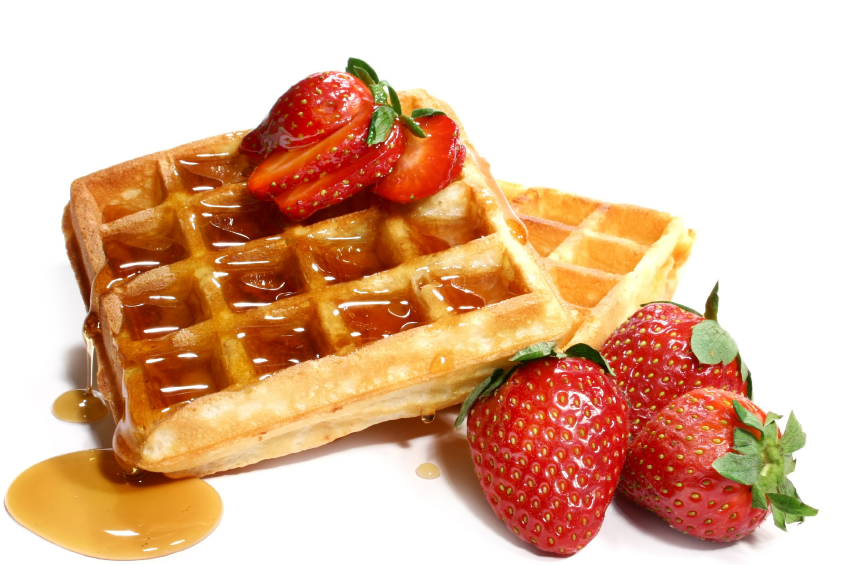
\includegraphics[scale=0.75]{pics/waffles.eps}
\end{center}
\vspace*{\fill}


\subsection{Filesystem backup}
Example: WAFL (Write Anywhere File Layout)
\vspace*{\fill}
\begin{center}
	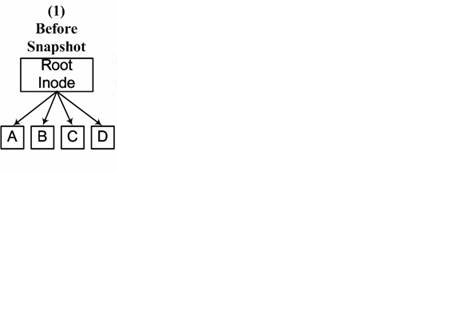
\includegraphics[scale=1.0]{pics/wafl0.eps}
\end{center}
\vspace*{\fill}


\subsection{Filesystem backup}
Example: WAFL (Write Anywhere File Layout)
\vspace*{\fill}
\begin{center}
	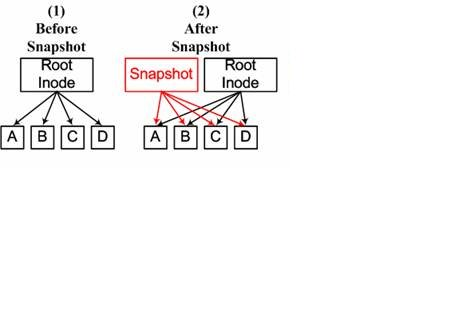
\includegraphics[scale=1.0]{pics/wafl1.eps}
\end{center}
\vspace*{\fill}


\subsection{Filesystem backup}
Example: WAFL (Write Anywhere File Layout)
\vspace*{\fill}
\begin{center}
	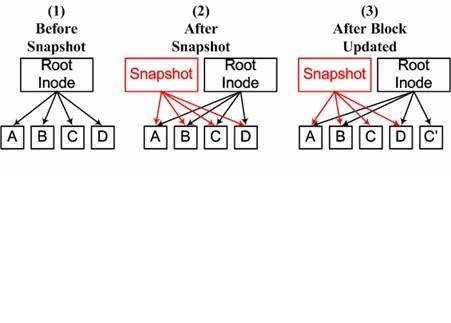
\includegraphics[scale=1.0]{pics/wafl2.eps}
\end{center}
\vspace*{\fill}


\subsection{Filesystem backup}
Example: WAFL (Write Anywhere File Layout)
\vspace*{\fill}
\begin{center}
	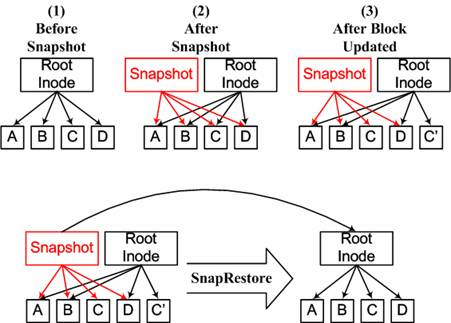
\includegraphics[scale=1.0]{pics/wafl.eps}
\end{center}
\vspace*{\fill}


\subsection{Filesystem backup}
Example: ZFS snapshots
\begin{itemize}
	\item ZFS uses a copy-on-write transactional object model (new data does
		not overwrite existing data, instead modifications are written to a
		new location with existing data being referenced), similar to WAFL
	\item a snapshot is a read-only copy of a file system (cheap and near
		instantaneous, due to CoW)
	\item initially consumes no additional disk space; the writable filesystem
		is made available as a ``clone''
	\item conceptually provides a branched view of the filesystem; normally
		only the ``active'' filesystem is writable
\end{itemize}

\subsection{ZFS Snapshots}
\smallish
\begin{verbatim}
$ pwd
/home/jschauma
$ ls -l .z*
ls: cannot access .z*: No such file or directory
$
\end{verbatim}
\Normalsize

\subsection{ZFS Snapshots}
\smallish
\begin{verbatim}
$ pwd
/home/jschauma
$ ls -l .z*
ls: cannot access .z*: No such file or directory
$ ls -lid .zfs
1 dr-xr-xr-x 3 root root 3 Jan 10  2013 .zfs
$
\end{verbatim}
\Normalsize

\subsection{ZFS Snapshots}
\smallish
\begin{verbatim}
$ pwd
/home/jschauma
$ ls -l .z*
ls: cannot access .z*: No such file or directory
$ ls -lid .zfs
1 dr-xr-xr-x 3 root root 3 Jan 10  2013 .zfs
$ ls -lai .zfs/snapshot
total 13
2 dr-xr-xr-x  4 root     root       4 Feb 28 21:00 .
1 dr-xr-xr-x  3 root     root       3 Jan 10  2013 ..
4 drwx--x--x 37 jschauma professor 88 Feb 24 22:32 amanda-_export_home_jschauma-0
4 drwx--x--x 37 jschauma professor 88 Feb 26 11:47 amanda-_export_home_jschauma-1
$
\end{verbatim}
\Normalsize

\subsection{ZFS Snapshots}
\smallish
\begin{verbatim}
$ pwd
/home/jschauma
$ ls -l .z*
ls: cannot access .z*: No such file or directory
$ ls -lid .zfs
1 dr-xr-xr-x 3 root root 3 Jan 10  2013 .zfs
$ ls -lai .zfs/snapshot
total 13
2 dr-xr-xr-x  4 root     root       4 Feb 28 21:00 .
1 dr-xr-xr-x  3 root     root       3 Jan 10  2013 ..
4 drwx--x--x 37 jschauma professor 88 Feb 24 22:32 amanda-_export_home_jschauma-0
4 drwx--x--x 37 jschauma professor 88 Feb 26 11:47 amanda-_export_home_jschauma-1
$ cd .zfs/snapshot
$ echo foo > amanda-_export_home_jschauma-0/oink
-ksh: amanda-_export_home_jschauma-0/oink: cannot create [Read-only file system]
$ ls -laid . /
2 dr-xr-xr-x  4 root root    4 Feb 28 21:00 .
2 drwxr-xr-x 26 root root 4096 Jan 27 11:44 /
\end{verbatim}
\Normalsize

\subsection{ZFS Snapshots}
\smallish
\begin{verbatim}
$ pwd
/home/jschauma/.zfs/snapshot
$ ls -lai amanda-_export_home_jschauma-0 >/tmp/a
$ ls -lai amanda-_export_home_jschauma-1 >/tmp/b
$ diff -bu /tmp/[ab]
--- /tmp/a	2014-03-01 22:55:49.000000000 -0500
+++ /tmp/b	2014-03-01 22:55:59.000000000 -0500
@@ -35,7 +35,7 @@
 57723 drwx------  3 jschauma professor         6 Dec 31 15:08 .subversion
 49431 -rw-------  1 jschauma professor         6 Dec 22 12:25 .sws.pid
    20 drwx------  2 jschauma professor         3 Jan 26 10:30 .vim
-61768 -rw-------  1 jschauma professor     14538 Feb 24 22:32 .viminfo
+61775 -rw-------  1 jschauma professor     14557 Feb 26 09:23 .viminfo
   173 -rw-------  1 jschauma professor      4355 Sep 17  2012 .vimrc
 45744 -rw-r--r--  1 jschauma professor         0 Jul 28  2013 .xsession-errors
    21 drwxr-xr-x  3 jschauma professor         6 Apr  4  2010 CS615A
$
\end{verbatim}
\Normalsize

\subsection{HW \#4}
Data backup to the cloud \\
\verb+https://www.cs.stevens.edu/~jschauma/615/s16-hw5.html+
\\
\verb+https://www.cs.stevens.edu/~jschauma/615/ec2-backup.txt+

\subsection{Reading}
Hurricane Sandy
\begin{itemize}
	\item \verb+http://is.gd/aaxzvI+
	\item \verb+http://is.gd/Y75pEA+
	\item \verb+http://is.gd/32Az7y+
	\item \verb+http://is.gd/FhAuFZ+
\end{itemize}

\subsection{Reading}
Manual Pages:
\begin{itemize}
	\item \verb+dump(8)+ and \verb+restore(8)+
\end{itemize}
Filesystem snapshots:
\begin{itemize}
	\item \verb+https://en.wikipedia.org/wiki/Snapshot_(computer_storage)+
	\item \verb+https://en.wikipedia.org/wiki/Time_Machine_(Apple_software)+
	\item \verb+http://comet.lehman.cuny.edu/jung/cmp426697/WAFL.pdf+
	\item \verb+http://www.cs.tau.ac.il/~ohadrode/slides/WAFL.pdf+
\end{itemize}
\vspace{.5in}
Book: \verb+http://www.oreilly.com/catalog/unixbr/+

\end{document}
